\documentclass[12pt, a4paper, oneside]{article}
\usepackage{astronotes}

\begin{document}

\pagestyle{fancy}
\fancyhf{}
\lhead{\textbf{กิตติพัศ พงศ์อรุโณทัย}\\{\today}}
\rhead{\textbf{Code_00}\\ชื่อเรื่อง}
\cfoot{\thepage}

\begin{titlepage}
    \centering
    
    %
\includegraphics[width=0.15\textwidth]{img/sklogo.png}
    %
\includegraphics[width=0.15\textwidth]{img/kvislogo.png}
    %
\includegraphics[width=0.15\textwidth]{img/mwitlogo.png}
    %
\includegraphics[width=0.15\textwidth]{img/mzpfp1.jpg}
    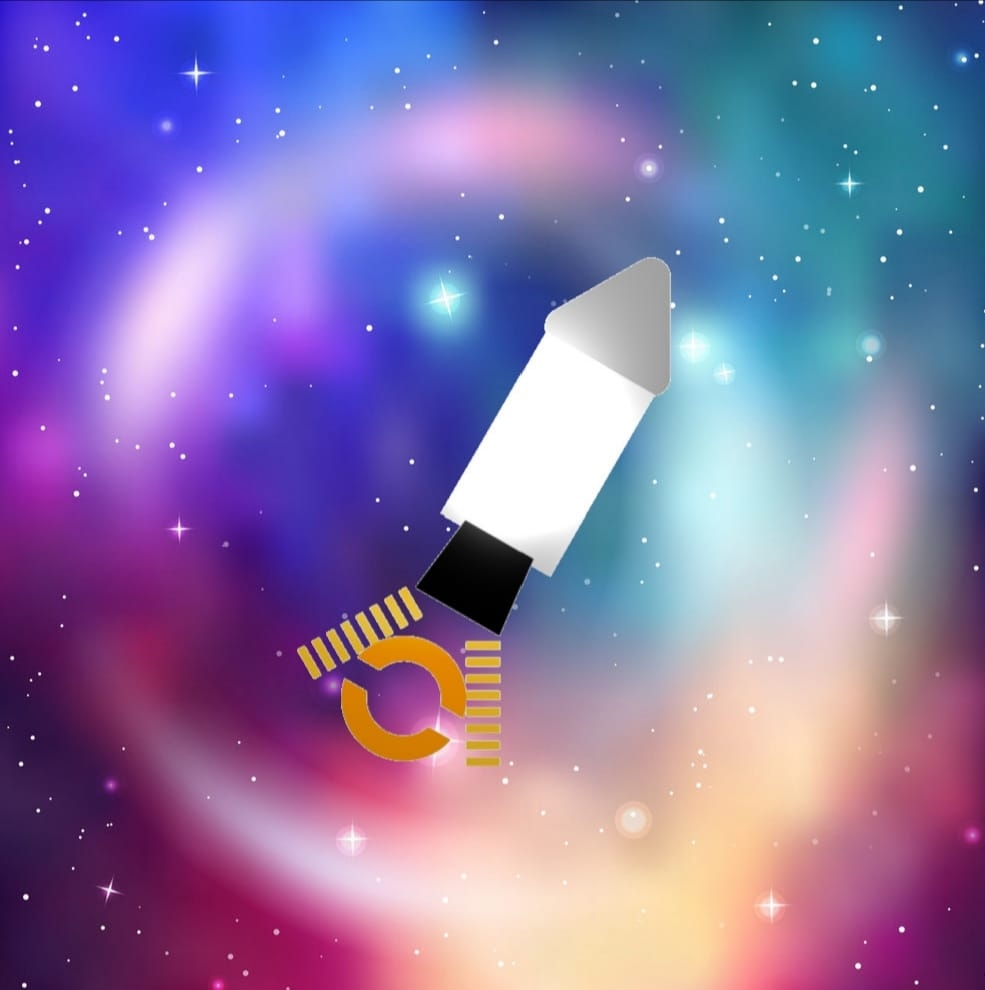
\includegraphics[width=0.15\textwidth]{img/mzpfp2.jpg}
    \par\vspace{1cm}
	{\Large \textsc{Astronomy POSN Summaries (AstroNotes)}\par}
    \vspace{0.25cm}
	{\Large \textsc{ไฟล์สรุปสำหรับ สอวน. ดาราศาสตร์}\par}

	\vspace{2cm}
	{\LARGE\bfseries Name\par}
    \vspace{0.25cm}
    {\LARGE\bfseries ชื่อเรื่อง\par}

	\vspace{1cm}
	{\Large\itshape กิตติพัศ พงศ์อรุโณทัย\par}
    \vspace{0.25cm}
    {\large\itshape โรงเรียนกำเนิดวิทย์\par}
    {\itshape ศูนย์ สอวน. ดาราศาสตร์ โรงเรียนมหิดลวิทยานุสรณ์ และโรงเรียนสวนกุหลาบวิทยาลัย}
	\vfill
% Bottom of the page
	{\large \today\par}
\end{titlepage}

\section{Section Name}
Section text

\end{document}
